%!TEX program = pdflatex
%----------------------------------------------------------------------------------------------------------------------
% Author: Charlotte Christiansen, Jonas Nygaard Eriksen, and Stig Vinther Møller
% Encoding: UTF8
% LaTeX File for "Forecasting US Recessions: The Role of Sentiment" 
% Last modified: September, 2015
%----------------------------------------------------------------------------------------------------------------------
% PREAMBLE
%----------------------------------------------------------------------------------------------------------------------

% Require the nag package to warn about obsolete stuff
\RequirePackage[l2tabu,orthodox]{nag}

% Setting document class, font, font size, and bibliography options
\documentclass[12pt,a4paper,onecolumn,oneside,notitlepage]{article}
\usepackage[left=2.5cm,right=2.5cm,top=2.5cm,bottom=2.5cm]{geometry}
\usepackage[onehalfspacing]{setspace}

% Setting bibliography and typography options
\usepackage[longnamesfirst]{natbib}
\usepackage[english]{babel}
\usepackage[utf8]{inputenc}
\usepackage{eucal}
\usepackage[T1]{fontenc}
\usepackage{hyphenat}
\usepackage{microtype}
\usepackage{verbatim}

% Loading math packages
\usepackage{amsmath}
\usepackage{amsfonts}
\usepackage{amssymb}
\usepackage{amsthm}

% Loading tables and figures packages
\usepackage{makeidx}
\usepackage{tabularx}
\usepackage{graphicx}
\usepackage{epstopdf}
\usepackage{booktabs}
\usepackage{lscape}
\usepackage{longtable}
\usepackage{seqsplit}
\usepackage{rotating}
\usepackage{multicol}

% Loading auxiliary packages
\usepackage{soul}
\usepackage{blindtext}
\usepackage{appendix}
\usepackage{todonotes}

% Setting caption options
\usepackage{caption}
\usepackage{subcaption}
\captionsetup{
    labelfont = bf,
    labelsep = colon
}

% Setting coloring of links and references
\usepackage{hyperref}
\usepackage{xcolor}
\definecolor{halfgray}{gray}{0.55} 
\definecolor{webgreen}{rgb}{0,.5,0}
\definecolor{webbrown}{rgb}{.6,0,0}
\definecolor{Maroon}{cmyk}{0, 0.87, 0.68, 0.32}
\definecolor{darkred}{RGB}{151,4,12}
\definecolor{dark_red}{RGB}{153,0,78}
\definecolor{navy_blue}{RGB}{0,0,128}
\definecolor{bluish_blue}{RGB}{18 128 171}
\definecolor{prettygreen}{RGB}{25 145 25}
\definecolor{prettybrown}{rgb}{0.737,0.353,0.396}
\definecolor{AUblue}{rgb}{0.02,0.24,0.45}
\hypersetup{
    colorlinks=true,
    breaklinks=true,
    bookmarksnumbered=true,
    bookmarksopen=true,
    bookmarksdepth=2,
    citecolor=navy_blue,
    linkcolor=navy_blue,
    urlcolor=prettybrown,
    pdftitle={Forecasting US Recessions: The Role of Sentiment},
    pdfauthor={Charlotte Christiansen, Jonas Nygaard Eriksen, and Stig Vinther Møller}
}

% Setting up values for table creation
\renewcommand{\arraystretch}{0.95}
\newcolumntype{Y}{>{\centering\arraybackslash}X}
\newcolumntype{Z}{>{\raggedright\arraybackslash}X}

% SETTING BIBLIOGRAPHY PROPERTIES
\setlength{\bibsep}{0.1pt plus 0.3ex}

%----------------------------------------------------------------------------------------------------------------------
% FRONT MATTER
%----------------------------------------------------------------------------------------------------------------------

\begin{document}

% Defining title and footnotes
\newcommand{\mytitle}{\textbf{\Large{Forecasting US Recessions: The Role of Sentiment \\ Figures and Tables}}}
\pagenumbering{arabic}
\renewcommand{\refname}{References}
\long\def\symbolfootnote[#1]#2{%
    \begingroup\def\thefootnote{%
        \fnsymbol{footnote}
    }\footnote[#1]{#2}\endgroup
}

% Setting up custom title page
\begin{titlepage}

    \thispagestyle{empty}
    \setlength{\parindent}{0cm}
    \begin{center}

        \small
        \renewcommand{\thefootnote}{\fnsymbol{footnote}}

        \vspace*{5cm} 
        \mytitle\symbolfootnote[1]{
            For comments and suggestions, we thank two anonymous referees, conference participants at the 2013 IFABS meeting in Nottingham, the 2013 CFE conference in London, the 2013 Nordic Finance Network meeting in Aarhus, and seminar participants at CREATES and Lund University. The authors acknowledge support from CREATES - Center for Research in Econometric Analysis of Time Series  DNRF78), funded by the Danish National Research Foundation.
        }

        \vspace{2cm}
        \textbf{\normalsize
            {Charlotte Christiansen}\symbolfootnote[2]{CREATES, Department of Economics and Business Economics, Aarhus University, Fuglesangs All{\'e} 4, DK-8210 Aarhus V, Denmark. Phone: +45 8716 5576. Email: \href{mailto:cchristiansen@econ.au.dk}{cchristiansen@econ.au.dk}.}  \hspace{0.2cm}
            {Jonas Nygaard Eriksen}\symbolfootnote[3]{CREATES, Department of Economics and Business Economics, Aarhus University, Fuglesangs All{\'e} 4, DK-8210 Aarhus V, Denmark. Phone: +45 8716 5321. E-mail: \href{mailto:jeriksen@econ.au.dk}{jeriksen@econ.au.dk}.}  \hspace{0.2cm}
            {Stig Vinther Møller}\symbolfootnote[7]{CREATES, Department of Economics and Business Economics, Aarhus University, Fuglesangs All{\'e} 4, DK-8210 Aarhus V, Denmark. Phone: +45 8716 4825. Email: \href{mailto:svm@econ.au.dk}{svm@econ.au.dk}.}
        }

        \vspace{1.2cm}
        {
            \normalsize  
            \vspace{1.5cm}
            This version: \today
        }
        \clearpage
        \thispagestyle{empty}
        \vspace*{2cm}
        \mytitle
        \vspace*{0.5cm}
        \begin{singlespace}
            \begin{abstract}
                \noindent We study the role of sentiment variables as predictors for US recessions. We combine sentiment variables with either classical recession predictors or common factors based on a large panel of macroeconomic and financial variables. Sentiment variables hold vast predictive power for US recessions in excess of both the classical recession predictors and the common factors. The strong importance of the sentiment variables is documented both in-sample and out-of-sample.\\\bigskip
                \noindent\textbf{Keywords:} Business cycles, Forecasting, Factor analysis, Probit model, Sentiment variables\\\medskip
                \noindent\textbf{JEL Classification:} C22, C25, E32, E37, G17. \\\bigskip
                \noindent\textbf{This version:} \today
            \end{abstract}
        \end{singlespace}
    \end{center}        
\end{titlepage}

%----------------------------------------------------------------------------------------------------------------------
% FIGURES
%----------------------------------------------------------------------------------------------------------------------

\clearpage
\begin{figure}[htbp]
    \caption{
        \textbf{Business and consumer confidence.} \newline 
        This figure plots the time series of business confidence (PMI$_{t}$; solid line) and consumer confidence (CC$_{t}$; broken line) against NBER defined recession dates in gray shading.
    }
    \centering
    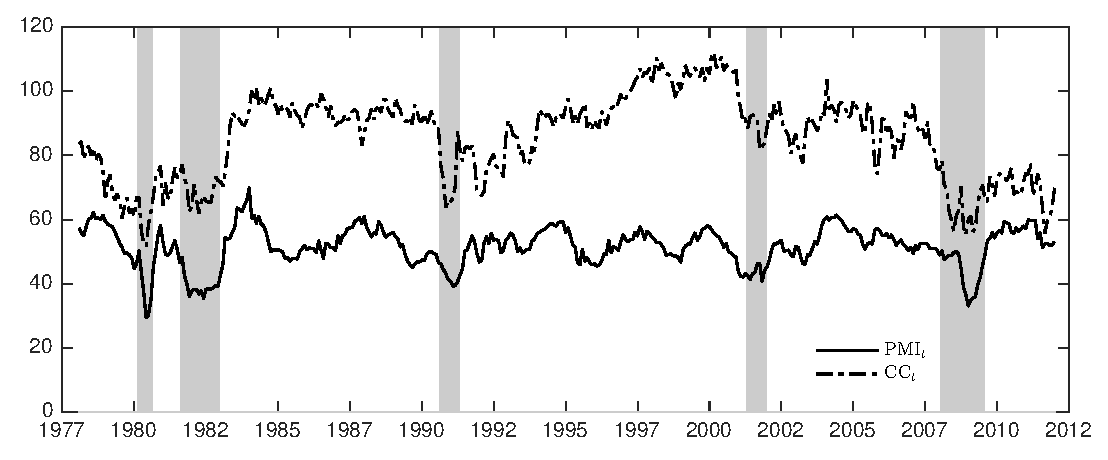
\includegraphics[width=\textwidth]{Figures/Figure1.eps} 
    \label{fig:busconindex}
\end{figure}

\clearpage
\begin{figure}[htbp]
    \caption{
        \textbf{In-sample fit.} \newline 
        This figure plots in-sample recession probabilities implied by selected models from Table 3. NBER defined recession dates are in gray shading.
    }
    \centering
    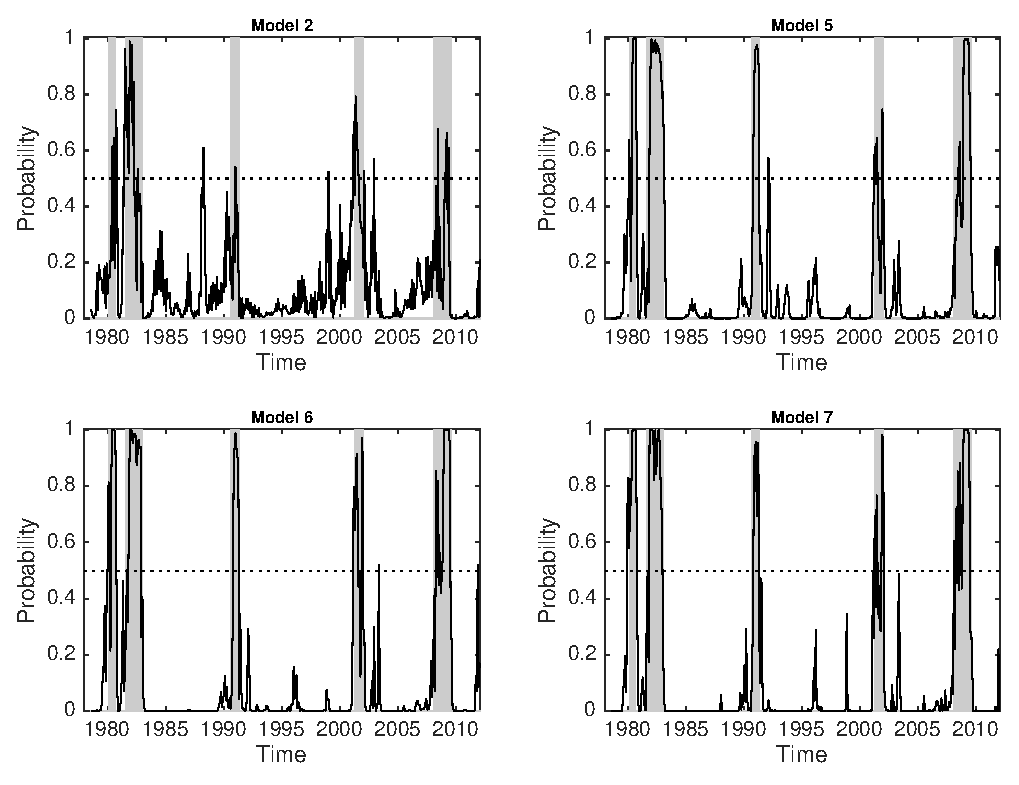
\includegraphics[scale=1]{Figures/Figure2.eps} 
     \label{fig:isfit}
\end{figure}

\clearpage
\begin{figure}[htbp]
    \caption{
        \textbf{In-sample ROC curves.} \newline 
        This figure plots in-sample ROC curves for selected models from Table 3. The 45 degree line represents a coin-toss classifier.
    }
    \centering
    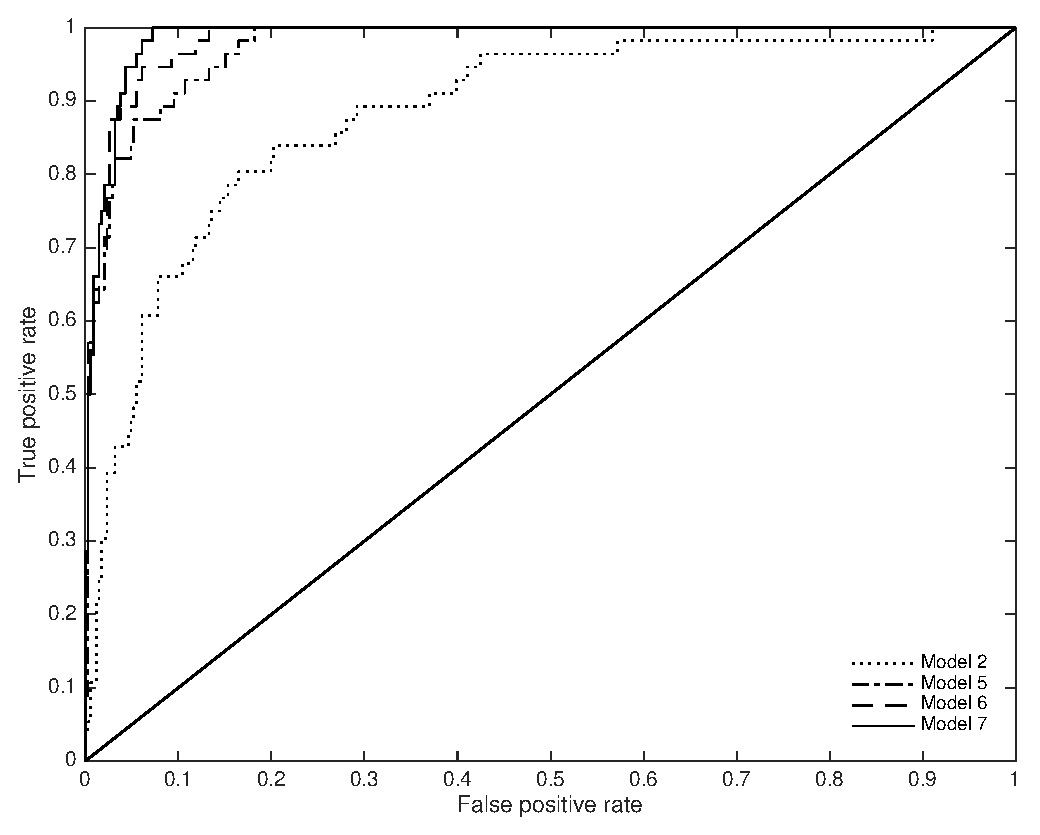
\includegraphics[scale=1]{Figures/Figure4.eps} 
    \label{fig:isroc}
\end{figure}

\clearpage
\begin{figure}[htbp]
    \caption{
        \textbf{Out-of-sample fit.} \newline 
        This figure plots out-of-sample recession probabilities implied by selected models from Table 4 for a one-month forecast horizon. NBER defined recession dates are in gray shading.
    }
    \centering
    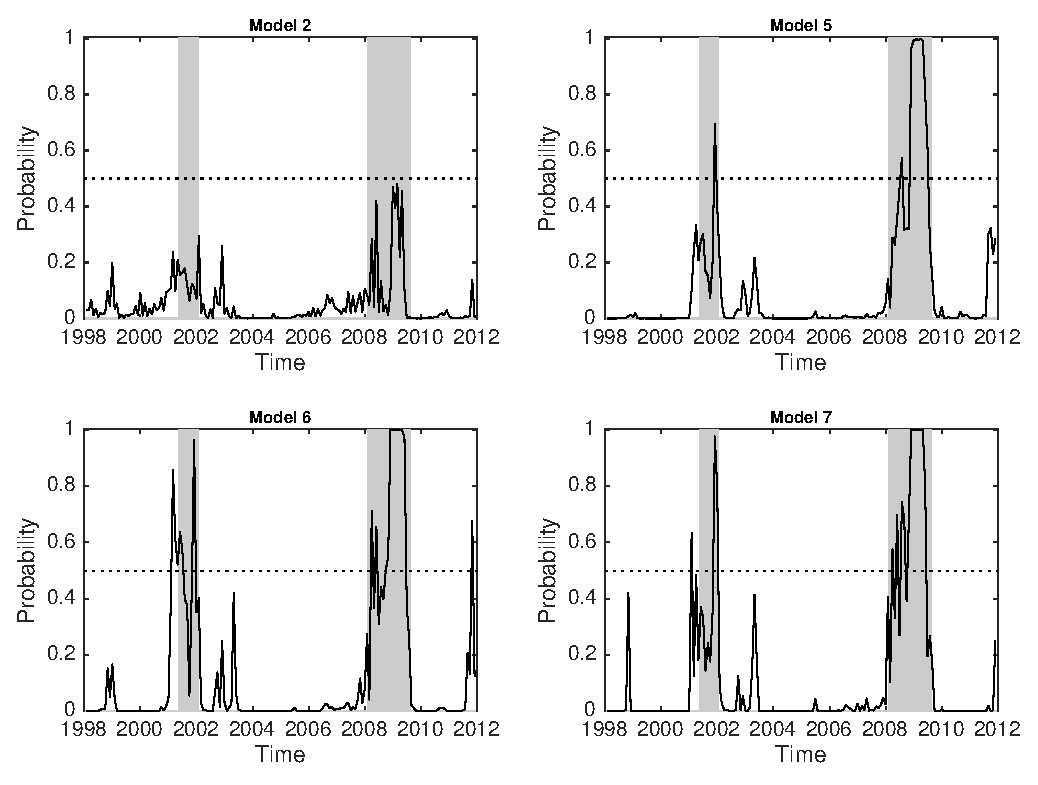
\includegraphics[scale=1]{Figures/Figure3_1.eps} 
    \label{fig:oosfit}
\end{figure}

%----------------------------------------------------------------------------------------------------------------------
% TABLES
%----------------------------------------------------------------------------------------------------------------------

\clearpage
\begin{table}[htbp]
    \centering
    \footnotesize
    \caption{
        \textbf{Correlations.} \newline 
        This table presents correlation coefficients between PMI$_{t}$ and CC$_{t}$ and the control variables used in the paper. The sample period is 1978:M1 to 2011:M12.
    }
    \begin{tabularx}{\textwidth}{YZZZZZZZ}
        \toprule
        Variable & PMI$_{t-1}$ & CC$_{t-1}$ & Variable & PMI$_{t-1}$ & CC$_{t-1}$ \\\midrule
TS$_{t-1}$ & 0.15 & -0.06 & $\hat{f}_{7,t-1}$ & 0.09 & 0.07 \\
FFR$_{t-1}$ & -0.20 & -0.08 & $\hat{f}_{8,t-1}$ & -0.03 & -0.12 \\
RET$_{t-1}$ & -0.05 & -0.04 & $\hat{f}_{9,t-1}$ & -0.01 & 0.12 \\
$\hat{f}_{1,t-1}$ & -0.02 & 0.03 & $\hat{f}_{10,t-1}$ & 0.02 & -0.09 \\
$\hat{f}_{2,t-1}$ & -0.64 & -0.42 & $\hat{f}_{11,t-1}$ & -0.13 & 0.03 \\
$\hat{f}_{3,t-1}$ & -0.38 & -0.59 & $\hat{f}_{12,t-1}$ & -0.10 & 0.02 \\
$\hat{f}_{4,t-1}$ & -0.16 & 0.11 & $\hat{f}_{13,t-1}$ & -0.05 & 0.06 \\
$\hat{f}_{5,t-1}$ & -0.09 & 0.11 & $\hat{f}_{14,t-1}$ & -0.01 & -0.02 \\
$\hat{f}_{6,t-1}$ & 0.24 & -0.30 & $\hat{f}_{15,t-1}$ & -0.00 & -0.02 \\


        \bottomrule
    \end{tabularx}
    \label{tab:cormat}
\end{table}

\clearpage
\begin{table}[htbp]
    \centering
    \footnotesize
    \caption{
        \textbf{The predictive ability of individual variables.} \newline 
        This table presents in-sample results from estimating univariate probit models at their preferred lag length selected using the BIC. The models are ranked according to their pseudo-R$^{2}$. LPS denotes the log probability score. AUC is the area under the ROC curve and the p-value refers to the null of no classification ability. The sample period is 1978:M1 to 2011:M12.
    }
    \begin{tabularx}{\textwidth}{YYYYYYYY}
        \toprule
        Rank & Variable & pseudo-R$^{2}$ & BIC & LPS & AUC & p-val \\\midrule
1 & PMI$_{t-1}$ & 0.47 & 80.14 & 0.18 & 0.95 & (0.00) \\
2 & CC$_{t-1}$ & 0.26 & 117.29 & 0.28 & 0.87 & (0.00) \\
3 & $\hat{f}_{2,t-1}$ & 0.23 & 123.23 & 0.29 & 0.84 & (0.00) \\
4 & $\hat{f}_{3,t-2}$ & 0.15 & 138.87 & 0.33 & 0.81 & (0.00) \\
5 & TS$_{t-6}$ & 0.09 & 151.10 & 0.36 & 0.73 & (0.00) \\
6 & FFR$_{t-6}$ & 0.07 & 154.49 & 0.37 & 0.65 & (0.00) \\
7 & $\hat{f}_{1,t-4}$ & 0.05 & 158.54 & 0.38 & 0.66 & (0.00) \\
8 & $\hat{f}_{6,t-6}$ & 0.04 & 160.85 & 0.39 & 0.66 & (0.00) \\
9 & $\hat{f}_{7,t-6}$ & 0.03 & 162.01 & 0.39 & 0.63 & (0.00) \\
10 & RET$_{t-4}$ & 0.03 & 162.29 & 0.39 & 0.61 & (0.00) \\
11 & $\hat{f}_{8,t-5}$ & 0.02 & 164.03 & 0.39 & 0.64 & (0.00) \\
12 & $\hat{f}_{14,t-2}$ & 0.02 & 164.75 & 0.39 & 0.58 & (0.03) \\
13 & $\hat{f}_{10,t-4}$ & 0.01 & 166.90 & 0.40 & 0.58 & (0.03) \\
14 & $\hat{f}_{13,t-1}$ & 0.01 & 167.12 & 0.40 & 0.57 & (0.05) \\
15 & $\hat{f}_{12,t-1}$ & 0.00 & 167.29 & 0.40 & 0.55 & (0.11) \\
16 & $\hat{f}_{15,t-4}$ & 0.00 & 167.30 & 0.40 & 0.57 & (0.06) \\
17 & $\hat{f}_{9,t-6}$ & 0.00 & 167.66 & 0.40 & 0.57 & (0.04) \\
18 & $\hat{f}_{4,t-2}$ & 0.00 & 167.79 & 0.40 & 0.52 & (0.32) \\
19 & $\hat{f}_{11,t-1}$ & 0.00 & 167.92 & 0.40 & 0.53 & (0.26) \\
20 & $\hat{f}_{5,t-5}$ & 0.00 & 168.21 & 0.40 & 0.48 & (0.72) \\


        \bottomrule
    \end{tabularx}
    \label{tab:top20is}
\end{table}

\clearpage
\begin{table}[htbp]
    \centering
    \footnotesize
    \caption{
        \textbf{In-sample estimation of various probit models.} \newline 
        This table presents in-sample results from estimating various probit models. Model composition is based on the BIC. \cite{KauppiSaikkonen2008} standard errors are reported in parentheses. log-$\mathcal{L}$ is the value of the log likelihood function, pseudo-R$^{2}$ is the \cite{Estrella1998} measure, and LPS denotes the log probability score. AUC is the area under the ROC curve and the p-value refers to the null of no classification ability. The sample period is 1978:M1 to 2011:M12.
    }
    \begin{tabularx}{\textwidth}{lYYYYYYYYYYY}
        \toprule
        Variable & Model 1 & Model 2 & Model 3 & Model 4 & Model 5 & Model 6 & Model 7 \\\midrule
PMI$_{t-1}$ &  &  & -0.24 &  & -0.22 & -0.23 & -0.28 \\
 &  &  & (0.03) &  & (0.04) & (0.05) & (0.05) \\
CC$_{t-1}$ &  &  &  & -0.07 & -0.08 & -0.06 & -0.08 \\
 &  &  &  & (0.01) & (0.02) & (0.02) & (0.02) \\
CC$_{t-6}$ &  &  &  &  & 0.04 &  &  \\
 &  &  &  &  & (0.02) &  &  \\
TS$_{t-6}$ & -0.35 & -0.14 &  &  &  & -0.33 &  \\
 & (0.10) & (0.12) &  &  &  & (0.12) &  \\
FFR$_{t-6}$ &  & 0.19 &  &  &  &  &  \\
 &  & (0.06) &  &  &  &  &  \\
RET$_{t-2}$ &  & -0.08 &  &  &  & -0.11 &  \\
 &  & (0.03) &  &  &  & (0.03) &  \\
RET$_{t-4}$ &  & -0.12 &  &  &  & -0.08 &  \\
 &  & (0.03) &  &  &  & (0.03) &  \\
RET$_{t-6}$ &  & -0.10 &  &  &  &  &  \\
 &  & (0.03) &  &  &  &  &  \\
$\hat{f}_{1,t-2}$ &  &  &  &  &  &  & -0.50 \\
 &  &  &  &  &  &  & (0.12) \\
$\hat{f}_{6,t-6}$ &  &  &  &  &  &  & -0.80 \\
 &  &  &  &  &  &  & (0.22) \\
$\hat{f}_{14,t-4}$ &  &  &  &  &  &  & 0.42 \\
 &  &  &  &  &  &  & (0.17) \\
log-$\mathcal{L}$ & -145.11 & -110.30 & -74.15 & -111.29 & -57.95 & -47.44 & -42.53 \\
pseudo-R$^{2}$ & 0.09 & 0.27 & 0.47 & 0.26 & 0.56 & 0.63 & 0.66 \\
BIC & 151.10 & 128.29 & 80.14 & 117.29 & 69.95 & 65.43 & 60.52 \\
LPS & 0.36 & 0.27 & 0.18 & 0.28 & 0.14 & 0.12 & 0.11 \\
CR50\% & 0.02 & 0.38 & 0.66 & 0.30 & 0.66 & 0.71 & 0.75 \\
CE50\% & 0.99 & 0.98 & 0.98 & 0.97 & 0.98 & 0.98 & 0.98 \\
AUC & 0.73 & 0.88 & 0.95 & 0.87 & 0.97 & 0.98 & 0.99 \\
p-val & (0.00) & (0.00) & (0.00) & (0.00) & (0.00) & (0.00) & (0.00) \\


        \bottomrule
    \end{tabularx}
    \label{tab:ISprobit}
\end{table}

\clearpage
\begin{table}[htbp]
    \centering
    \footnotesize
    \caption{
        \textbf{Out-of-sample results.} \newline 
        This table presents out-of-sample results for the main models. The forecasting horizons range from one month to twelve months. Pseudo-R$^{2}$ is the \cite{Estrella1998} measure and LPS denotes the log probability score. AUC is the area under the ROC curve and the p-value refers to the null of no classification ability. The out-of-sample window runs from 1998:M1 to 2011:M12.
    }
    \begin{tabularx}{\textwidth}{lYYYYYcYYYYYYYYYYYYYYY}
        \toprule
         & 1 & 3 & 6 & 9 & 12 &  & 1 & 3 & 6 & 9 & 12 \\\midrule
 & \multicolumn{5}{c}{\textit{pseudo-R$^{2}$}} &  & \multicolumn{5}{c}{\textit{LPS}} \\\cmidrule{2-6}\cmidrule{8-12}
Model 1 & -0.04 & 0.01 & 0.14 & 0.22 & 0.28 &  & 0.47 & 0.45 & 0.39 & 0.36 & 0.34 \\
Model 2 & 0.07 & 0.25 & 0.30 & 0.22 & 0.21 &  & 0.41 & 0.33 & 0.32 & 0.36 & 0.38 \\
Model 3 & 0.45 & 0.39 & 0.26 & 0.11 & 0.05 &  & 0.23 & 0.27 & 0.34 & 0.42 & 0.45 \\
Model 4 & 0.19 & 0.21 & 0.14 & 0.05 & -0.01 &  & 0.35 & 0.35 & 0.40 & 0.45 & 0.48 \\
Model 5 & 0.57 & 0.48 & 0.31 & 0.11 & -0.05 &  & 0.18 & 0.22 & 0.31 & 0.42 & 0.51 \\
Model 6 & 0.59 & 0.58 & 0.49 & 0.32 & 0.27 &  & 0.17 & 0.18 & 0.23 & 0.31 & 0.35 \\
Model 7 & 0.64 & 0.56 & 0.31 & 0.15 & 0.07 &  & 0.15 & 0.19 & 0.31 & 0.40 & 0.44 \\\cmidrule{2-6}\cmidrule{8-12}

 & \multicolumn{5}{c}{\textit{AUC}} &  & \multicolumn{5}{c}{\textit{p-val}} \\\cmidrule{2-6}\cmidrule{8-12}
Model 1 & 0.56 & 0.65 & 0.76 & 0.82 & 0.84 &  & 0.16 & 0.01 & 0.00 & 0.00 & 0.00 \\
Model 2 & 0.84 & 0.90 & 0.90 & 0.87 & 0.87 &  & 0.00 & 0.00 & 0.00 & 0.00 & 0.00 \\
Model 3 & 0.96 & 0.93 & 0.88 & 0.77 & 0.64 &  & 0.00 & 0.00 & 0.00 & 0.00 & 0.01 \\
Model 4 & 0.81 & 0.78 & 0.73 & 0.65 & 0.56 &  & 0.00 & 0.00 & 0.00 & 0.01 & 0.16 \\
Model 5 & 0.98 & 0.96 & 0.90 & 0.73 & 0.53 &  & 0.00 & 0.00 & 0.00 & 0.00 & 0.31 \\
Model 6 & 0.97 & 0.98 & 0.95 & 0.88 & 0.85 &  & 0.00 & 0.00 & 0.00 & 0.00 & 0.00 \\
Model 7 & 0.98 & 0.97 & 0.91 & 0.77 & 0.68 &  & 0.00 & 0.00 & 0.00 & 0.00 & 0.00 \\


        \bottomrule
    \end{tabularx}
    \label{tab:OOSprobit}
\end{table}

\clearpage
\begin{table}[htbp]
    \centering
    \footnotesize
    \caption{
        \textbf{Dynamic probit models.} \newline 
        This table report in-sample results from estimating dynamic probit models. Dynamic 5 is the dynamic probit model equivalent of model 5, dynamic 6 is the dynamic version of model 6, and dynamic 7 of model 7. The choice of explanatory variables is based on the BIC. See notes to Table 3 for remaining entries.
    }
    \begin{tabularx}{\textwidth}{lYYYYYYYYYYYYYYYYYYYYYYY}
        \toprule
        Variable & Dynamic 1 & Dynamic 2 & Dynamic 3 \\\midrule
PMI$_{t-1}$ & -0.19 & -0.18 & -0.24 \\
 & (0.04) & (0.05) & (0.05) \\
CC$_{t-1}$ & -0.09 & -0.06 & -0.07 \\
 & (0.02) & (0.02) & (0.02) \\
CC$_{t-5}$ & 0.06 &  &  \\
 & (0.02) &  &  \\
TS$_{t-6}$ &  & -0.39 &  \\
 &  & (0.14) &  \\
RET$_{t-2}$ &  & -0.12 &  \\
 &  & (0.03) &  \\
RET$_{t-4}$ &  & -0.07 &  \\
 &  & (0.03) &  \\
$\hat{f}_{1,t-2}$ &  &  & -0.54 \\
 &  &  & (0.11) \\
$\hat{f}_{6,t-6}$ &  &  & -0.76 \\
 &  &  & (0.21) \\
$\hat{f}_{14,t-4}$ &  &  & 0.48 \\
 &  &  & (0.19) \\
y$_{t-3}$ & 0.88 & 0.95 & 0.71 \\
 & (0.55) & (0.48) & (0.47) \\
log-$\mathcal{L}$ & -55.01 & -44.35 & -40.98 \\
pseudo-R$^{2}$ & 0.58 & 0.65 & 0.67 \\
BIC & 70.00 & 65.34 & 61.96 \\
LPS & 0.14 & 0.11 & 0.10 \\
CR50\% & 0.71 & 0.80 & 0.82 \\
CE50\% & 0.98 & 0.98 & 0.98 \\
AUC & 0.98 & 0.98 & 0.99 \\
p-val & (0.00) & (0.00) & (0.00) \\


        \bottomrule
    \end{tabularx}
    \label{tab:dynprobit}
\end{table}

\clearpage
\begin{table}[htbp]
    \centering
    \footnotesize
    \caption{
        \textbf{Stability tests for unknown break points.} \newline 
        This table presents \cite{Andrews1993} tests for a single structural change at an unknown location. The sup of the Lagrange multiplier (LM) statistic is taken over an interior portion that excludes 25\% of the sample at each end point. The critical values are obtained from \cite{Estrella2003}.
    }
    \begin{tabularx}{\textwidth}{lYYYYYYYYYY}
        \toprule
         & $\sup$-LM$_{t}\left(\omega\right)$ & CV & H$_{0}$; No break \\\midrule
Model 1 & 5.37 & 10.96 & Not rejected \\
Model 2 & 10.04 & 19.30 & Not rejected \\
Model 3 & 7.15 & 10.96 & Not rejected \\
Model 4 & 3.25 & 10.96 & Not rejected \\
Model 5 & 8.28 & 15.45 & Not rejected \\
Model 6 & 8.84 & 19.30 & Not rejected \\
Model 7 & 9.90 & 19.30 & Not rejected \\


        \bottomrule
    \end{tabularx}
    \label{tab:stabilitytest}
\end{table}

\clearpage
\begin{table}[htbp]
    \centering
    \footnotesize
    \caption{
        \textbf{Forecasting industrial production growth.} \newline 
        This table presents in-sample results from forecasting one-month ahead industrial production growth (in logs) using various linear regression models. Model composition is based on the BIC. Newey-West standard errors are reported in parentheses. The sup of the \cite{Andrews1993} LR$_{T}\left(\omega\right)$ statistic is taken over an interior portion of the sample that excludes 25\% of the observations at each end point with p-values obtained using the method from \cite{Hansen1997} in parentheses. The sample period is 1978:M1 to 2011:M12.
    }
    \begin{tabularx}{\textwidth}{lYYYYYYYYYYYYYYYYY}
        \toprule
        Variable & Model 1 & Model 2 & Model 3 & Model 4 & Model 5 & Model 6 & Model 7 \\ \midrule 
PMI$_{t-1}$ &  &  & 0.05 &  & 0.10 & 0.09 & 0.09 \\ &  &  & (0.01) &  & (0.01) & (0.01) & (0.01) \\PMI$_{t-3}$ &  &  &  &  & -0.06 & -0.06 & -0.06 \\ &  &  &  &  & (0.01) & (0.01) & (0.01) \\CC$_{t-1}$ &  &  &  & 0.02 & 0.01 & 0.01 & 0.01 \\ &  &  &  & (0.00) & (0.00) & (0.00) & (0.00) \\TS$_{t-4}$ & 0.09 & 0.03 &  &  &  &  &  \\ & (0.03) & (0.03) &  &  &  &  &  \\FFR$_{t-4}$ &  & -0.05 &  &  &  &  &  \\ &  & (0.01) &  &  &  &  &  \\RET$_{t-2}$ &  & 0.03 &  &  &  & 0.02 &  \\ &  & (0.01) &  &  &  & (0.01) &  \\RET$_{t-3}$ &  & 0.04 &  &  &  &  &  \\ &  & (0.01) &  &  &  &  &  \\RET$_{t-6}$ &  & 0.04 &  &  &  & 0.02 &  \\ &  & (0.01) &  &  &  & (0.01) &  \\$\hat{f}_{1,t-3}$ &  &  &  &  &  &  & 0.10 \\ &  &  &  &  &  &  & (0.03) \\$\hat{f}_{6,t-6}$ &  &  &  &  &  &  & 0.05 \\ &  &  &  &  &  &  & (0.03) \\BIC & -0.73 & -0.83 & -0.95 & -0.81 & -1.07 & -1.10 & -1.07 \\adj. R$^{2}$ & 0.03 & 0.17 & 0.22 & 0.10 & 0.33 & 0.36 & 0.35 \\

        sup-LR$_{T}\left(\omega\right)$ & 6.01 & 5.48 & 7.65 & 4.70 & 4.41 & 1.57 & 2.37  \\
        p-val & (0.03) & (0.00) & (0.01) & (0.09) & (0.02) & (0.64) & (0.22)  \\
        \bottomrule
    \end{tabularx}
    \label{tab:ipgrowth}
\end{table}


%----------------------------------------------------------------------------------------------------------------------
% BIBLIOGRAPHY
%----------------------------------------------------------------------------------------------------------------------

\newpage 
\bibliographystyle{elsarticle-harv}
\bibliography{cem_refs}

\end{document}

%----------------------------------------------------------------------------------------------------------------------
% END OF LATEX DOCUMENT
%----------------------------------------------------------------------------------------------------------------------